%	% ****** Start of file MolecularSpinFlipLoss.tex ******
%
%
%

\documentclass[%
 reprint,
%superscriptaddress,
%groupedaddress,
%unsortedaddress,
%runinaddress,
%frontmatterverbose,
%preprint,
%showpacs,preprintnumbers,
%nofootinbib,
%nobibnotes,
%bibnotes,
 amsmath,amssymb,
 aps,
%prl,
pra,
%prb,
%rmp,
%prstab,
%prstper,
%floatfix,
]{revtex4-1}

\usepackage{graphicx}% Include figure files
\usepackage{dcolumn}% Align table columns on decimal point
\usepackage{bm}% bold math
\usepackage[hidelinks]{hyperref}% add hypertext capabilities
%\usepackage[mathlines]{lineno}% Enable numbering of text and display math
%\linenumbers\relax % Commence numbering lines
\usepackage{textcomp}

\usepackage{color}
\newcommand{\red}[1]{{\color{black} #1}}

% Define new commands for common phrases and standardized typesetting
\newcommand{\exmple}{This is an Example.}



\begin{document}

\title{Supplementary Material for ``New Voltage Configurations for Enhanced Stark Deceleration''}%

\author{David Reens}
\thanks{dave.reens@colorado.edu.}

\author{Hao Wu}
\author{Alexander Aeppli}
\author{Anna McAuliffe}
\author{Piotr Wcis\l o}
\author{Tim Langen}%
\altaffiliation{Present Address: 5. Physikalisches Institut and Center for Integrated Quantum Science and Technology (IQST), Universit\"at Stuttgart, Pfaffenwaldring 57, 70569 Stuttgart, Germany}

\author{Jun Ye}
\affiliation{JILA, National Institute of Standards and Technology and the University of Colorado and\\ Department of Physics, University of Colorado, Boulder, Colorado 80309-0440, USA}


\date{\today}

%%%%%%%%%%%%%%%%%%%%%
% OUTLINE 
%%%%%%%%%%%%%%%%%%%%%
% Introduction
% Effective Moving Trap
% Alternate Charging Technique
% Experimental Validation
% Further Simulation Results


%%%%%%%%%%%%%%%%%%%%%
% ABSTRACT
%%%%%%%%%%%%%%%%%%%%%
\begin{abstract}
We expand upon our primary result in several key areas of lesser importance for the general audience. These include a full derivation of the effective moving potential for molecules in a pulsed Stark decelerator, a thorough treatment of the problem of spin-flip losses induced by the new voltage configurations, some discussion of technical aspects of the definition and utilization of new operating modes, and some discussion of extensions to these techniques.
\end{abstract}

\maketitle


%%%%%%%%%%%%%%%%%%%%%%%%%%%%%%%%%
%     The Effective Moving Trap
%%%%%%%%%%%%%%%%%%%%%%%%%%%%%%%%%
\section{Effective Moving Trap Derivation\label{sec:effpot}}
We can derive the effective moving trap in 3D as follows:
\begin{equation}
m\ddot{x}=\frac{\partial V}{\partial x}\approx \frac{\partial}{\partial x}\frac{1}{2t_0}\int\limits_{t-t_0}^{t+t_0}V(x(t),t)dt
\end{equation}
\begin{equation}
W(x,y,\bar{z}) = \frac{1}{2\pi}\int\limits_{z_0+\bar{z}}^{z_0+L+\bar{z}}V(x,y,z)dz, 
\end{equation}
Copied out of the main text:
\begin{equation}
W(x,y,z^*) = - maz^* + \frac{1}{L}\int\limits_{z^*}^{z^*+L}V(x,y,z) dz,
\end{equation}
with $W$ the effective potential energy defined in coordinates relative to the synchronous molecule at the center of the effective moving trap, $V$ the potential energy in real space coordinates, $L$ the length of a deceleration stage, $a$ the average acceleration experienced by the synchronous molecule, $m$ the mass of a molecule, and a longitudinal coordinate $z$ which has $z=0$ at the location where the synchronous molecule sits during a switching event.

where $z$ points along the decelerator axis, $V$ is the lab-frame potential energy induced via the Stark effect on the molecule and applied during propagation of the synchronous molecule from position $z_0$ to $z_0+L$, and $\bar{z}$ is the non-inertial transform from the lab-frame: 
\begin{equation}
\bar{z} = z + v_0 t - \frac{1}{2}a t^2.
\end{equation}

\begin{multline}
W(x,y,z^*) = - maz^* + 
\frac{1}{L'}\!\!\int\limits_{z^*}^{z^*+L'}\!\!V'(x,y,z) dz \\
+\frac{1}{L-L'}\!\!\int\limits_{z^*+L'}^{z^*+L}\!\!V(x,y,z) dz,\hspace{2cm}
\end{multline}
where $V'$ represents the lab-frame Stark potential induced by the alternative charge configuration, and $L'$ gives twice the distance required for the synchronous molecule to fly from its longitudinal position during a switch event, to the center of the approaching pin pair which would have been grounded under S=1 operation. This hardly changes the longitudinal behavior of the device, but adds significant transverse depth to the effective moving trap.


%\begin{figure}[t]
%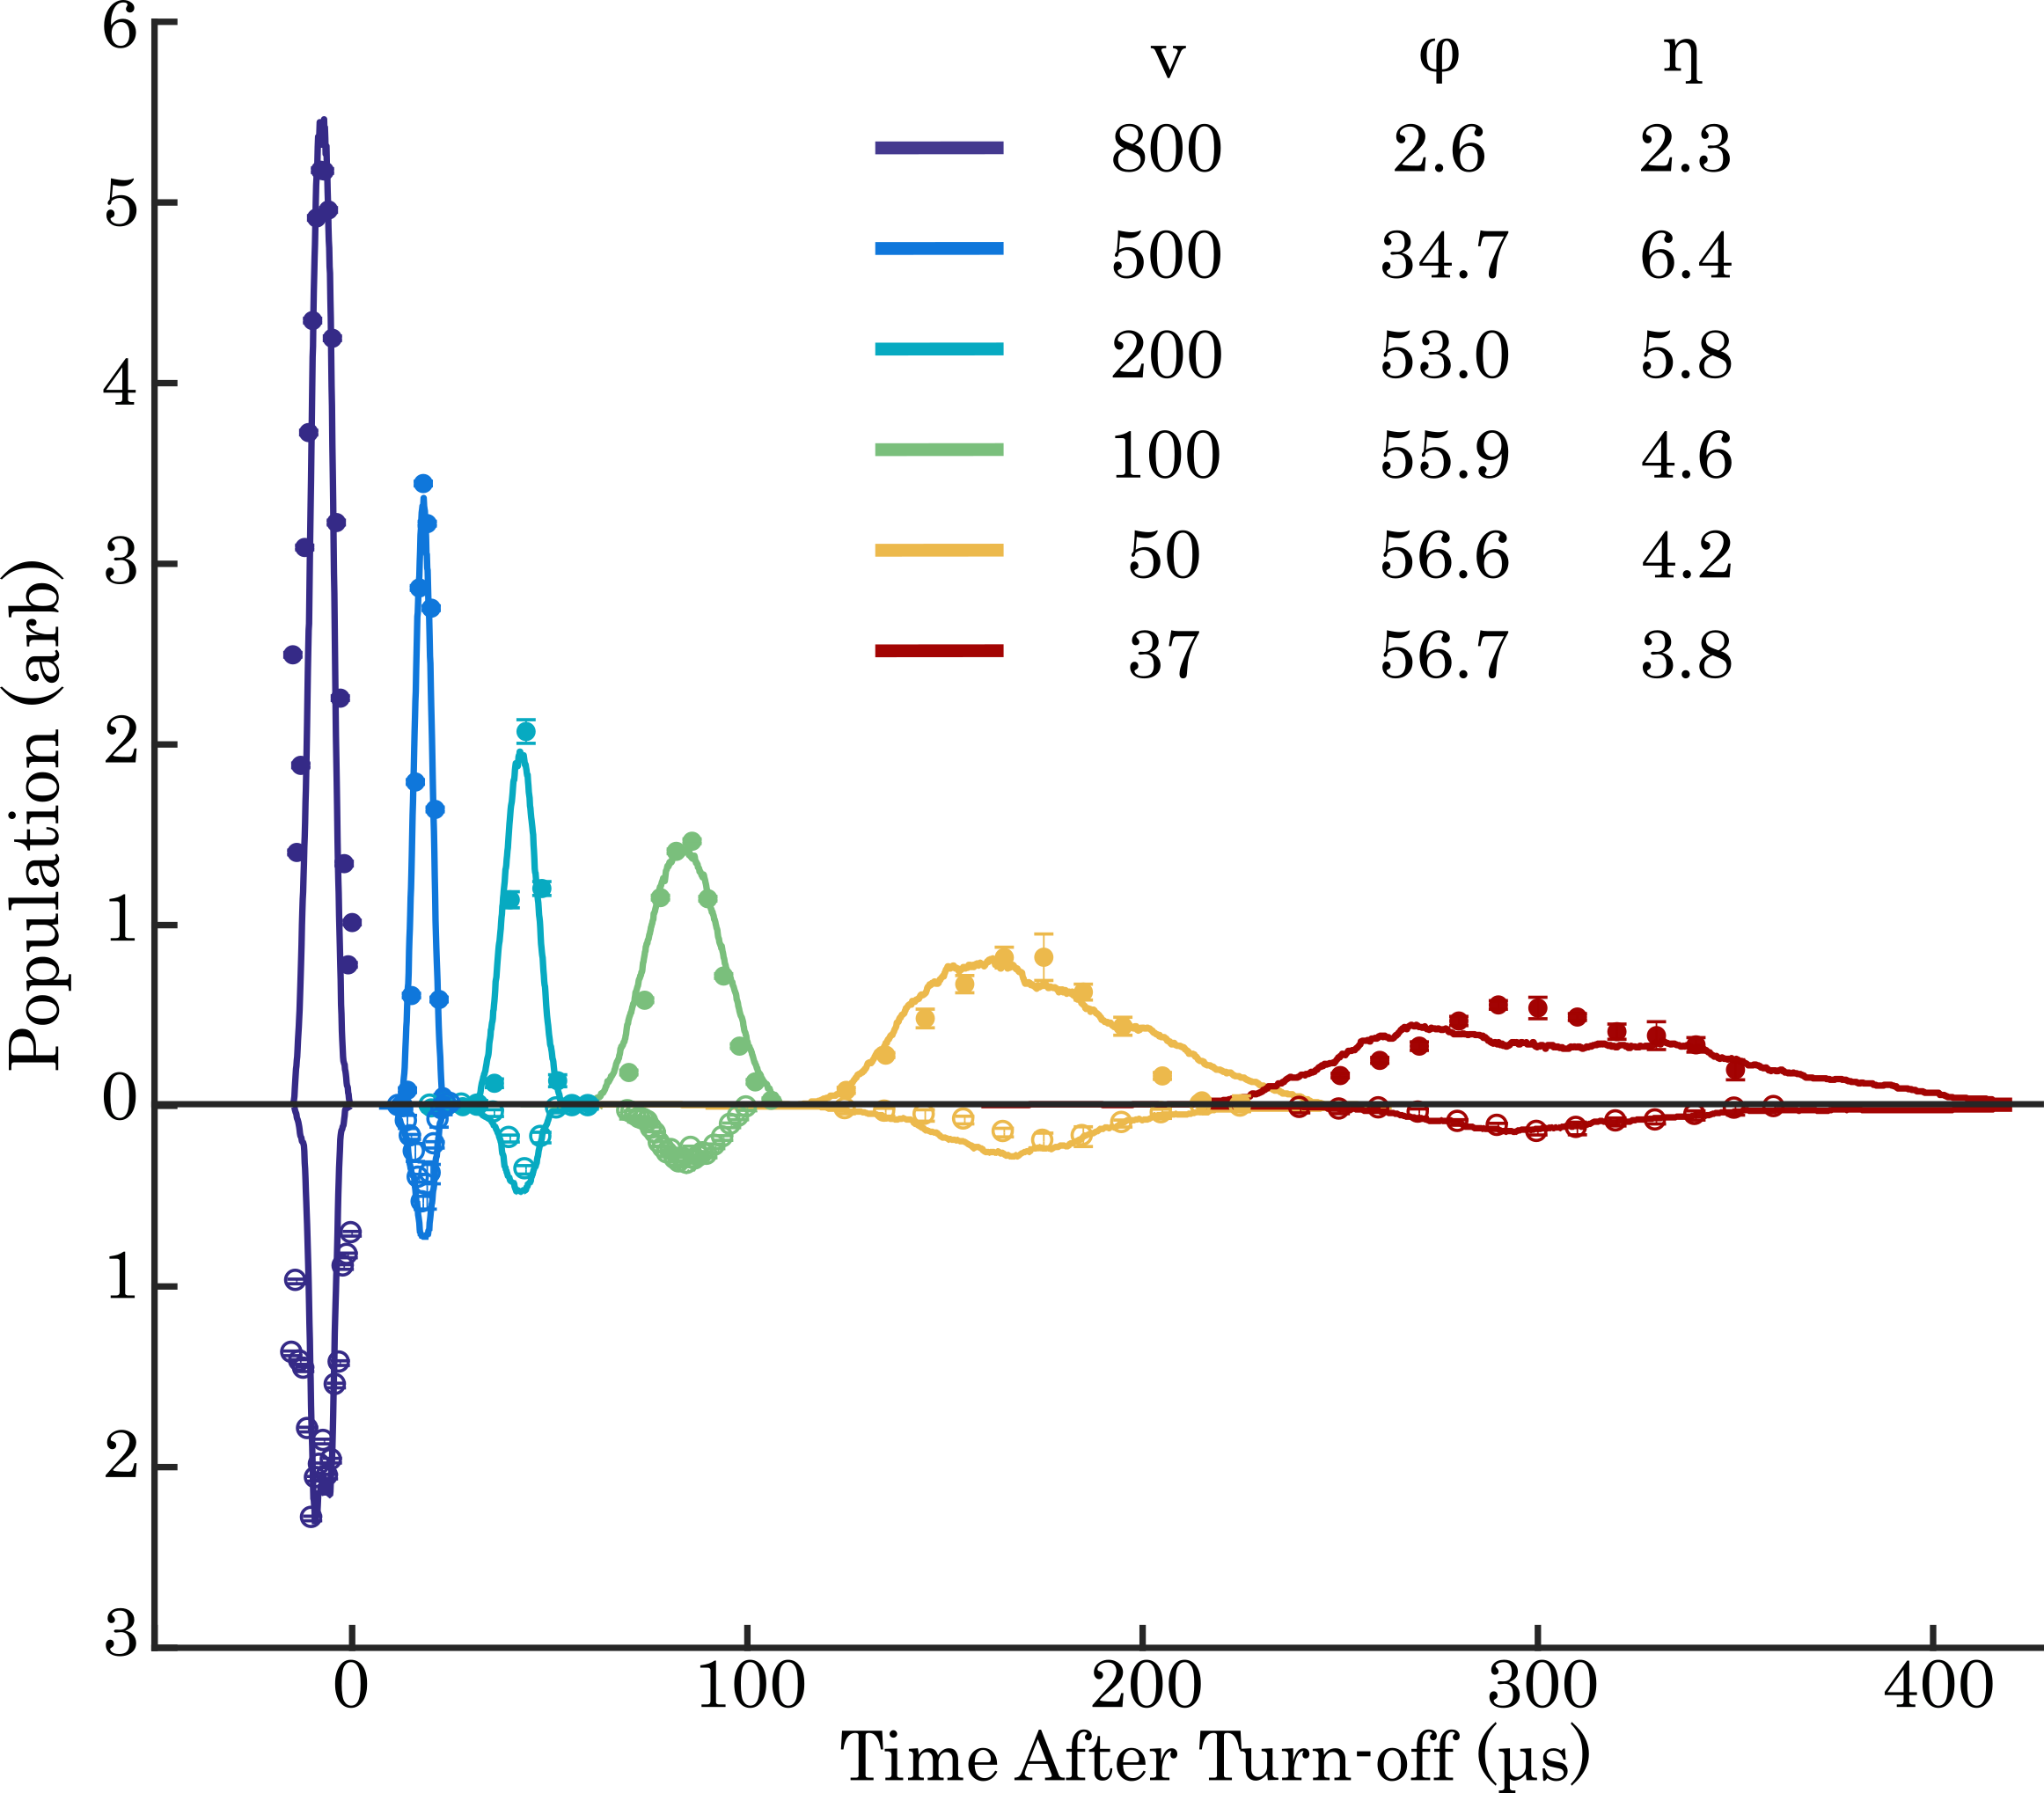
\includegraphics[width=\linewidth]{speedvary.png}%
%
%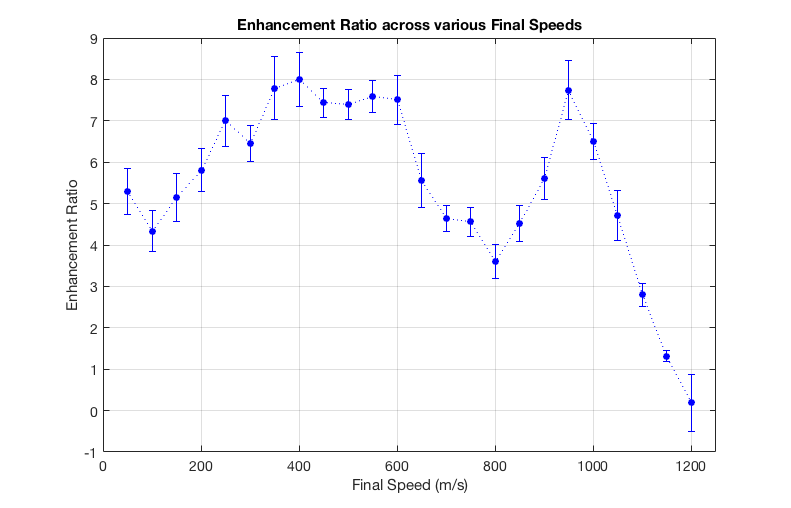
\includegraphics[width=\linewidth]{Data/ratio-combined.png}%
%\label{fig:speedvary}
%\caption{
%(a). Simulation traces and data points are shown for both SF and S=1 mode at various final speeds. 
%The data are collected with a $333$ stage decelerator and a beam of OH radicals expanded in Neon at an initial speed of $820\text{ m/s}$. 
%The ratio $\eta$ of peak detected molecules between SF and S=1 are listed for each speed. 
%It is seen that large gains persist even down to final speeds appropriate for trap loading.
%(b).~Efficiency as a function of final speed. Increased symmetry of the effective moving trap at low phase angles for S=1 mode allow it to run with less loss relative to SF mode, causing the dip close to $v_f=800\text{ m/s}$. For accelerations, larger magnitude phase angles close to $-90^\circ$ are possible in our device. Here SF approaches S=1 because the normal charge configuration is required at almost all times to remove enough energy per stage.
%}
%\end{figure}

%It is important to make our results applicable to devices with different lengths. 
%For this purpose, we can run our decelerator in a hybrid mode designed to simulate shorter lengths by first bunching the molecules and then slowing them. 
%We fix the phase angle for slowing in all cases, so as to effectively study the enhancement between S=1 and SF as a function of hold time in the effective moving trap. 
%The results are shown in Fig.~\ref{fig:holdtime}. 
%Even for a very short decelerator designed to use Xenon buffer gas and slow close to rest, a total hold-time of $2\text{ ms}$ still results in a factor of $2.5$ enhancement by using SF mode.

%We also study the behavior of molecules in their effective moving traps at long times, see Fig.~\ref{fig:longtimes}.
%This allows us to distinguish several effects. 
%The very long-time asymptotic trapped number is a direct reflection of the effective moving trap depth.
%The time-scale for approach to this asymptotic number is a measure of the ergodicity of the effective trap.
%It is seen that in S=1 mode nearly all are lost eventually, as expected.
%It is also seen that while traveling wave geometries sport increased trap-depths, their asymmetry and increased ergodicity relative to VSF mode makes the latter preferable for a wide range of run-times useful in typical experiments.


%\section{Discussion}
%It is important to reconcile our language thus far with the notion of the phase space conservative behavior of non-dissipative Hamiltonian systems such as Stark decelerators. While it is true in theory that such systems cannot compress or dilute phase space; in practice the conserved volume can become hopelessly swirled about, so that any reasonable scientific device, which typically accepts an approximately ellipsoidal phase space volume, inevitably includes a mixture of conserved and non-conserved volumes, so that the final phase space density can be severely diluted. Simply put, a trap with a hole in it is certainly a non-dissipative Hamiltonian system, but that doesn't prevent molecules falling out.

\section{Non-Adiabatic Transitions}
Non-adiabatic transitions are important in the context of these alternate deceleration modes, because the charge configurations used for boosting transverse confinement feature quadrupolar field arrangements with electric field minima and rapid field rotation close to those minima.
This situation makes possible transitions that preserve parity but change the $m$ quantum number describing the alignment of the molecule with the field.
Molecular states chosen for Stark deceleration typically feature total $J>1/2$, in which case there exist states with less than maximal $|m|$ to which transitions can occur resulting in dramatically reduced strength of Stark forces applied by the decelerator.
For the case of OH Molecules, $J=3/2$, and estimations of the magnitude of spin-flip transitions suggest that it could be as large as a $50\%$ effect in our device. 
However, in practice, deviations from the ideal geometry tend to greatly reduce the risk of spin-flip transitions, because for example slight nonzero angles between pins, or length differences, tend to cause the unintentional removal of electric field minima.
In our device, we find no detectable influence of spin-flip losses, based on good agreement between data and Monte Carlo without including their effect.
This could be ensured by intentionally unbalancing the lengths of pin-pairs, so that one pair has rods that are a few millimeters longer than the other. A $3$~mm imbalance would be sufficient to pull the electric field zero completely out of the flight path of the molecules. 

\section{Extensions}
Besides XSF mode, mentioned above, several other direct extensions of our results are worth mentioning. Firstly, at low phase angles, we note that it is in general not worth the effort to mix in configurations $A$ and $A'$ of Fig.~\ref{fig:chargecartoon}, and good results can be achieved with only ever having a single rod charged at a time as in SF Mode. In the case of VSF mode, one can quite efficiently run a decelerator at low phase angles with only a single HV switch, by switching between configuration $D$ and configuration $0$, where only a small orientation preserving voltage is applied.

For those interested in extending results in the direction of VSF mode but without tri-polar switches, gains can be made by admixing the configuration with all four rods charged to their normal voltages, also discussed as $\text{S}=3^+$ mode in Ref.~\cite{HudsonThesis2006}. Switching between the XSF configuration and the configuration with all pins charged at their normal voltages could be achieved with only two HV switches, and also affords XSF-like performance.

Even restricting attention to the SF and VSF modes discussed primarily in this work, there is the possibility of tuning when the alternate configurations are applied and for how long. 
We have studied this to some extent and found that applying the alternate configurations symmetrically about the grounded pin pair worked within 10\% of the optimum we could obtain by more carefully studying the space of possible timings.
In general however, one could imagine much more thoroughly studying the space of possibilities, and even introducing the possibility of using more than two different configurations within a single stage, as performed in Ref.~\cite{Zhang2016} but for the usual charge configurations.

Finally, we add that it may even be that a brand new electrode configuration is more well-suited for capitalizing on the gains afforded by the use of alternate charge configurations. The obvious direction would be to keep the pulsed design but somehow curve or change the pin arrangement so that the alternate configurations would feature even better focusing, without too dramatically reducing the magnitude of the large electric field that can be applied within a single stage in the usual configuration.


%includes uncited bib entries
%\nocite{*}
\bibliographystyle{apsrev4-1_no_Arxiv}
\bibliography{supplementary}



\end{document}
%
% ****** End of file MolecularMajoranaLoss.tex ******













